\begin{comment}
\begin{itemize}
  \item 2人の顔をウインドウで表示する代わりに,対面で人の横顔を見るような表示
  \item 横顔を表示することで,立体感を拡張させ,あたかも対面しているかのような状況を作り出す
  \item 今回は横顔の生成は実際の映像を用いては行っていない
  \item Unity上で3Dモデルを横から撮影し,UnityCapture\cite{8}を用いて仮想カメラの映像としてOpenCVで処理した
  \item 後述するおかしら会議\cite{10}のように,Unity内の球体に画像をマッピングして,疑似的に顔を生成し,横から撮影する
  というった方法も考えられる.
  \item 機械学習ベースの横顔生成手法としてYiboら\cite{11}の方法が挙げられる.
\end{itemize}

\begin{figure}[tp]
  \centering
  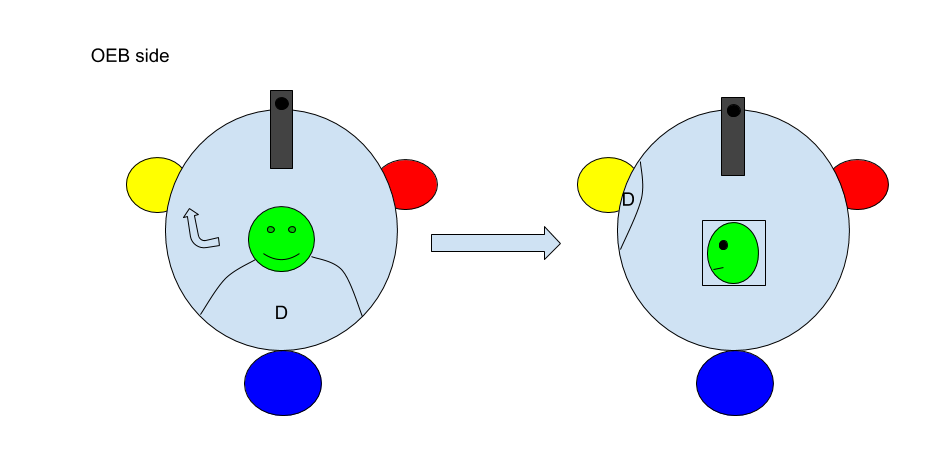
\includegraphics[scale=0.6]{fig/PCimgSlideYoko.png}
  \caption{OmniEyeBall上で,PC使用者の表示位置が移動する模式図}
\end{figure}
\end{comment}

6-2-1で会話中のビデオ会議参加者を表示する方法を提案した.本節では
立体的な映像を表示するという部分に着目し,小窓に横顔を
表示する方法を提案する.

\begin{figure}[tp]
  \centering
  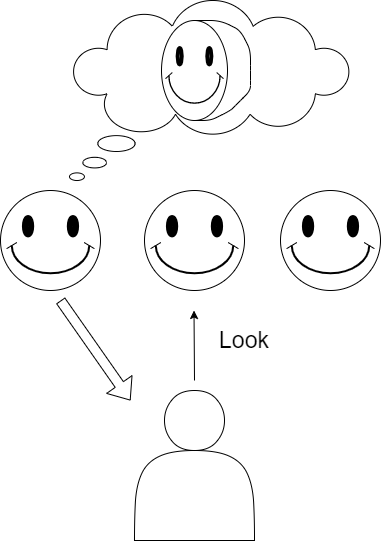
\includegraphics[scale=0.7]{fig/yokogao.png}
  \caption{横顔が見える状況} \label{yokogao}
\end{figure}

表\ref{yokogao}のように,複数人で対面している状況を考える.
話者が自身に話しかけていない場合,別の人物に顔を向けている
場合が多く,その際には話者の横顔が視認できる.
ここでは,小窓に話者の正面顔ではなく横顔を表示する
方法を提案する.対面時の立体的情報を再現することで,
ビデオ会議の参加者に更なる没入感を提供することが目的である.

実装時間の関係で,参加者の実際の顔の横顔を再現するには至らなかった.
このことは今後の課題とする.代用案として,昨今様々な場所で配布されており,
入手・仕様・作成が容易な3Dモデルを利用して,横顔を表示する手法を提案する.

3Dモデルの撮影にはUnity\cite{16}を用いた.UnityではOpenCV及びDlib
が利用可能で,Dlibで取得した顔のランドマーク情報から3Dモデルの体や表情を
動かすことが可能である.また,Unityでは自由にシーン描画カメラを配置することができる,
ここでは3Dモデルの左右にカメラを配置し,リアルタイムで横顔を撮影した.
Unity内カメラの映像はUnityCapture\cite{8}を利用することで,容易に
仮想カメラの映像として利用することが出来る.

\begin{figure}[tp]
  \centering
  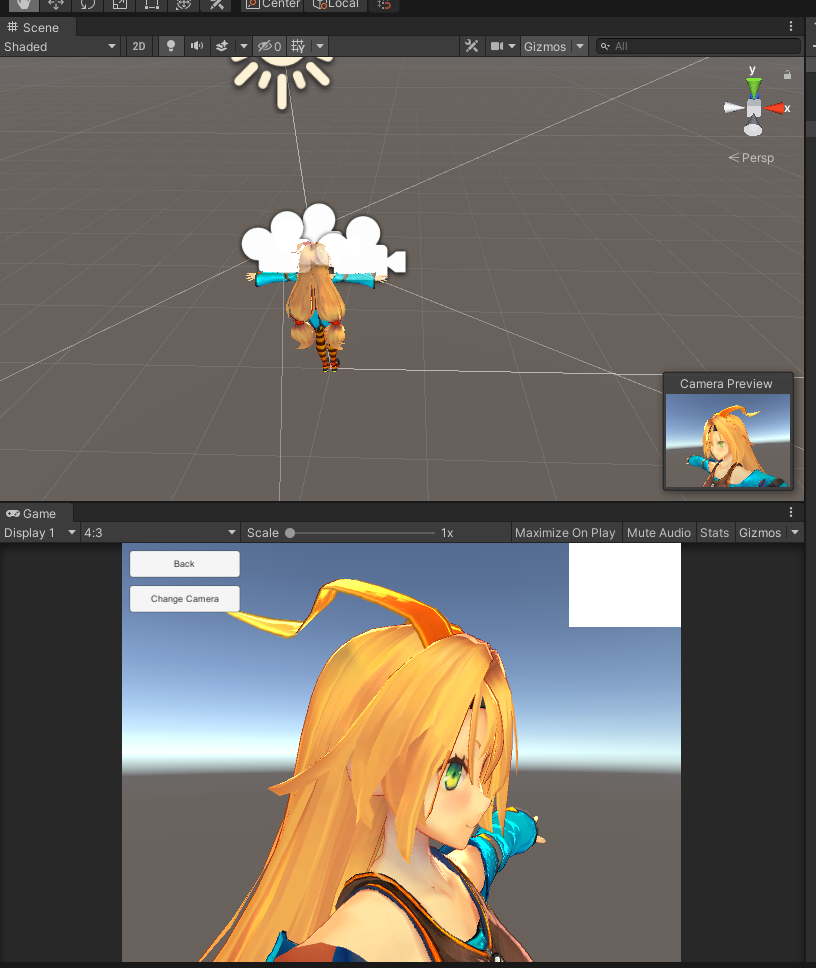
\includegraphics[scale=0.7]{fig/unitycam.png}
  \caption{3Dモデルを撮影する様子}
\end{figure}

\begin{figure}[tp]
  \centering
  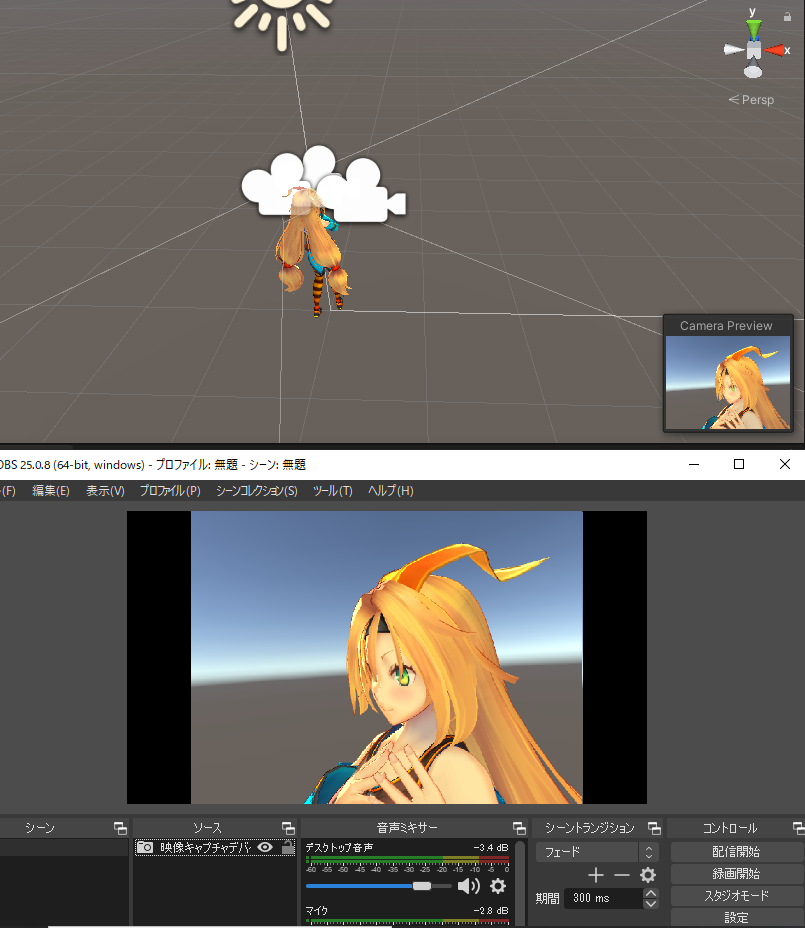
\includegraphics[scale=0.6]{fig/unitycapture.png}
  \caption{UnityCaptureを用いた他アプリケーションへの映像ストリーミング}
\end{figure}

通信の高速化のため,プロセス間通信で顔の位置情報を送信し,カメラを移動させる
ということは行わなかった.OmniEyeBallの使用者から見て,右側の参加者が見られているときには
左から見た横顔が,左側の参加者が見られているときには右から見た横顔が表示されるようにした.

\begin{figure}[tp]
  \centering
  \includegraphics[scale=0.2]{fig/yokoV.png}
  \caption{生成した横顔をOmniEyeBall上で表示させた様子}
\end{figure}

今後,ビデオ会議参加者自身の顔を生成する方法としては,
後述するおかしら会議\cite{10}の表示法を用いる手段がある.
Unity内の仮想球体にspriteとして,PC使用者の顔写真を張り付ける.
そうした球体を撮影することで,疑似的な顔写真を生成する.

機械学習ベースの方法として,横顔生成手法としてYiboら\cite{11}の方法が挙げられる.
これらの方法を用いた表示は,今後の研究課題とする.